You want to design an orientation controller for a satellite system whose thrusters provide a torque $\tau$ to modify the angular position $\theta$ with transfer function
\[
G(s)=\frac{\theta(s)}{\tau(s)}=\frac{0.1}{s^2}.
\]


\begin{center}
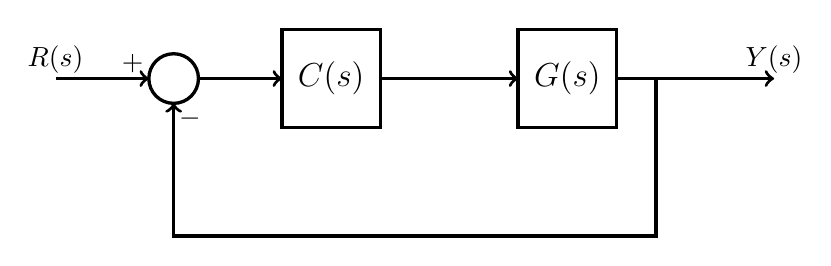
\begin{tikzpicture}[scale=1,inner sep=0pt,outer sep=0pt,very thick,
sysblock/.style={draw,rectangle,inner sep=2pt,minimum width=1.25cm,minimum height=1.25cm,very thick}]
\draw (1.5,0) node[draw,circle] (sum1) {$\rule{0pt}{18pt}$};
\draw (3.5,0) node[sysblock] (Kp) { \large $C(s)$};
\draw (6.5,0) node[sysblock] (G) {\large $G(s)$};
\draw[->] (0,0) node[above=2pt] {$R(s)$} -- (sum1.180) node[above left=2pt] {$+$};
\draw[->] (sum1.0) --  (Kp);
\draw[->] (Kp) -- (G.180);
\draw[->] (G.0) -- ++(2,0) node[above=2pt] {$Y(s)$};
\draw[->] (G.0) ++(0.5,0) -- ++(0,-2) -| (sum1.-90) node[below right=2pt] {$-$};
\end{tikzpicture}
\end{center}
You want to add damping to the system to minimize any oscillations (\%OS < 5\%) but still maintain a 1\% settling time of less than 60 s to a unit step input.

\begin{enumerate}[(a)]
\item Sketch the allowable pole locations in the complex plane to meet the \%OS and settling time requirements.
\item Which type of controller is more likely to improve the damping: PI or PD? Why?
\item Import your plant transfer function $G(s)$ into Matlab's sisotool and insert a real zero at an arbitrary value (if you answered PD) or a real pole at $0$ and a real zero at an arbitrary value (if you answered PI). Move your arbitrary zero and change your closed-loop gain until you have achieved the required specifications. Submit your root locus, your final $C(s)$, and your step response from sisotool (showing the specifications have been met) as part of your homework.
\end{enumerate}